\chapter{Techniques d'analyses de malwares}

Lors de l'analyse d'un logiciel suspect, le code source est rarement disponible
et le seul support de travail est l'exécutable fournit.
Pour appréhender son comportement, il est alors nécessaire de recourir à
l'utilisation de nombreux outils et astuces.\\

Il existe deux approches à l'étude d'exécutable au comportement inconnu:
l'analyse statique et l'analyse dynamique.\\
L'analyse statique consiste à examiner le binaire sans l'exécuter,
tandis que l'analyse dynamique se fait au cours de son exécution.
Ces deux approches sont en fait complémentaires et permettent d'obtenir
une vision d'ensemble sur le comportement du binaire étudié.

\section{Analyse statique}

L'analyse statique est donc une méthode d'étude reposant uniquement
sur la lecture du binaire, sans l'exécuter. Celle-ci se base sur l'étude
des propriétés du binaire, de son code assembleur et permet de récupérer
des informations sur l'élément suspect sans risquer de contaminer ou
de modifier de manière involontaire son environnement de travail.

\subsection{Scanner antivirus}

Une des premières et plus répandues techniques d'analyse,
quelles que soient les connaissances en informatiques,
est le passage par un antivirus. Celui-ci permet d'identifier,
neutraliser et même éliminer de nombreux logiciels malveillants.\\

Ils reposent principalement sur 3 techniques:
\begin{itemize}
\item[$\bullet$] {Comparaison des signatures virales;}
\item[$\bullet$] {Analyse du comportement des binaires suspectés;}
\item[$\bullet$] {Analyse de forme, à partir de règles regexp
  (très utilisés pour les mails).\\}
\end{itemize}

Si le logiciel incriminé est identifié, alors celui-ci est connu et
reconnu depuis déjà un certain temps par les bases de données des anti-virus:
des études devraient être disponibles sur le net.

\subsection{Hash du sample et comparaison aux bases de données}

Les signatures utilisées par les anti-virus sont des identifiants propres
à chaque binaire, à une portion de code ou à un comportement particulier.
Les techniques et heuristiques utilisées dépendent des types de scanner
mais vont du simple hash de binaire aux algorithmes d'analyse
de comportement. Cette dernière permet de trier les logiciels suspects
par familles, en fonction de leur comportement
(phishing, modification de registres, \ldots) mais aussi d'en analyser et
détecter certains qui sont alors encore inconnus, simplement par leurs actions.\\

Dans le cas de logiciels détectés comme malveillants mais encore inconnus,
de nouvelles signatures doivent être générées. En effet, bien que
le comportement soit détecté comme suspect, celui-ci n'est pas encore
totalement étudié et peut présenté des principes de protections
(comme de réplication par exemple) qu'il sera nécessaire de déterminer
afin de développer de nouveaux outils et de débarrasser totalement
les victimes de leurs charges virales.\\

\subsection{Examen de l'exécutable}

Quel que soit le binaire, celui-ci va fournir des informations relative
à son exécution, comme l'architecture supportée, la version (32/64 bits),
l'endianness, le point d'entrée (si celui-ci n'est pas le \textit{main}), \ldots
Ces informations ne sont pas stockées dans le corps du binaire mais
dans une en-tête, de manière différentes en fonction des types d'exécutables.
Mais les mêmes informations seront présentes, quels que soient
les supports utilisés.\\

Parmi les formats présents, les plus répandus sont les \textbf{ELF},
\textbf{PE} et \textbf{Mach-O}.\\

$\bullet$ ELF (Extensible Linking Format, ou plus formellement, Executable and
Linkable Format) est le format le plus présent dans les systèmes d'exploitation
de type Unix, excepté pour Mac OS X, permettant de représenter les exécutables,
les fichiers objets, les bibliothèques partagées comme les core dumps.\\

Les informations peuvent être récupérées par les fonctions \textit{file},
\textit{readelf}, \ldots
\begin{figure}[H]
\begin{verbatim}
$> readelf -h ch23
En-tête ELF:
  Magique:   7f 45 4c 46 01 01 01 00 00 00 00 00 00 00 00 00
  Classe:                            ELF32
  Données:                           complément à 2, système à octets de
poids faible d'abord (little endian)
  Version:                           1 (current)
  OS/ABI:                            UNIX - System V
  Version ABI:                       0
  Type:                              EXEC (fichier exécutable)
  Machine:                           Intel 80386
  Version:                           0x1
  Adresse du point d'entrée:         0x8048450
  Début des en-têtes de programme :  52 (octets dans le fichier)
  Début des en-têtes de section :    2404 (octets dans le fichier)
  [...]
\end{verbatim}
\caption {Données comprises dans l'en-tête d'un binaire ELF}
\end{figure}

D'autres informations peuvent être trouvées dans le binaire, notamment
les bibliothèques et fonctions importées/exportées.
Celles-ci sont extrêmement utiles pour l'analyse d'un binaire, afin d'avoir
une idée de son comportement sans l'exécuter.\\

$\bullet$ PE (Portable Executable) est le format de fichier des exécutable
et des bibliothèques sur les systèmes Windows. Il sert à décrire les binaires
(.exe), les bibliothèques dynamiques (.dll) et les pilotes (.sys).\\

Ces informations peuvent être récupérées de nombreuses manières.\\
Voici un extrait du résultat de la commande \textit{pedump}, sur Linux:
\begin{figure}[H]
\begin{verbatim}
$> pedump ch22.exe
PE Header:                                 NT Header:
	         Magic (0x010b): 0x010b           	   Image Base (0x400000): 0x00400000
	             LMajor (6): 0x0b             	Section Alignment (8192): 0x00002000
	             LMinor (0): 0x00             	   File Align (512/4096): 0x00000200
	              Code Size: 0x00003000       	            OS Major (4): 0x0004
	  Initialized Data Size: 0x00003400                                  [...]
	Uninitialized Data Size: 0x00000000
	        Entry Point RVA: 0x00004f3e
	 	  Code Base RVA: 0x00002000
		  Data Base RVA: 0x00006000
\end{verbatim}
\caption {Données comprises dans l'en-tête d'un binaire PE}
\end{figure}

$\bullet$ Mach-O pour les systèmes Mac OS X.

\subsection{Recherche de chaînes de caractères}

Une des manières d'analyser un exécutable est aussi d'observer les caractères
imprimables présents au milieu du code. En effet, si celui-ci n'est
pas obfusqué, les chaînes de caractères écrites "en brut" ou les fonctions
utilisées comme les sections peuvent être retrouvées assez facilement.
Avec la commande \textit{strings}, il est possible d'afficher toutes les chaînes
d'au moins 4 caractères ascii.

\begin{figure}[H]
\begin{verbatim}
$> /tmp/HB3$ strings ch23
/lib/ld-linux.so.2
__gmon_start__
libc.so.6
_IO_stdin_used
strncpy
__stack_chk_fail
printf
strlen
memset
__libc_start_main
[...]
Usage : %s <your name>
[...]
.init
.text
[...]
.data
.bss
[...]
main
_init
\end{verbatim}
\caption{Résultat de la commande \textit{strings} sur un binaire}
\end{figure}

Il est également possible d'utiliser d'autres outils comme \textit{nm},
qui peuvent fournir des informations supplémentaires comme le nom des fonctions
et librairies utilisées, ainsi que les variables globales utilisées.

\subsection{Packer et techniques de protection du binaire}

Mais l'analyse statique peut faire face à un certain nombre d'obstacles.
En effet, celle-ci repose essentiellement sur le principe de lecture de code
et en est donc entièrement dépendante.
Si le binaire se trouve, d'une quelconque manière, obfusqué, que son code est
modifié au cours de l'exécution ou simplement que les données originales sont
altérées, alors sa lecture et sa compréhension en seront bien réduites.

Ainsi, il est possible de se retrouver face à un logiciel que l'on va qualifier
de "packé" (TODO: check) ou de "stripped".
Cette partie s'attardera uniquement sur ceux obfusquant le comportement
du binaire, même si ils n'ont pas tous vocation à le faire (comme ceux se basant
uniquement sur un principe de compression de données).\\

Une de ces techniques consiste à chiffrer la charge utile, malveillante
(le .text ou le .data par exemple, à condition d'avoir les droits d'écriture
dans la région). Le code suspect est alors composé de la
routine de déchiffrement et du payload chiffré. La clef, quant à elle,
pourra être stockée dans la routine de déchiffrement, le payload ou encore
récupérée depuis l'extérieur: depuis un fichier ou par une requête
vers un serveur.

De même, il existe plusieurs méthodes de chiffrement, allant du
XOR à celles utilisant les courbes elliptiques, du chiffrement unique
aux chiffrés imbriqués, bloc par bloc ou du payload entier
(voir figure~\ref{packer}).\\

\begin{figure}[H]
\centering
\begin{tikzpicture}
  \draw[line width=.8pt] (0,0) -- (0,.8) -- (4,.8) -- (4,0) --cycle;
  \draw[line width=.8pt, pattern=checkerboard, pattern color=red!70]
  (1,0) -- (1,.8) -- (4,.8) -- (4,0) --cycle;
  \draw[<->, >=latex] (0,-.2) -- (1,-.2);
  \node[align=center] at (0.5,-.6){\shortstack{routine de\\déchiffrement}};
  \draw[->, >=latex] (0.65,.8) [out=90, in=90] to (2,.8);
  \node[align=center] at (1.7,1.8){
    \shortstack{déchiffre l'intégralité\\ du payload restant}};

  \draw[line width=.8pt] (6,0) -- (6,.8) -- (12,.8) -- (12,0) --cycle;
  \draw[line width=.8pt, pattern=checkerboard, pattern color=red!70]
  (7,0) -- (7,.8) -- (12,.8) -- (12,0) --cycle;
  \draw[line width=.8pt, fill=blue!70]
  (9.5,0) -- (9.5,.8) -- (12,.8) -- (12,0) --cycle;
  \draw[pattern=checkerboard, pattern color=red!70]
  (9.5,0) -- (9.5,.8) -- (12,.8) -- (12,0) --cycle;
  \draw[line width=.8pt, dashed] (12,.8) -- (13,.8);
  \draw[line width=.8pt, dashed] (12,0) -- (13,0);
  \draw[<->, >=latex] (6,-.2) -- (7,-.2);
  \node[align=center] at (6.5,-.6){\shortstack{routine de\\déchiffrement}};
  \draw[<->, >=latex] (8.5,-.2) -- (9.5,-.2);
  \node[align=center] at (9,-.6){\shortstack{routine de\\déchiffrement}};
  \draw[->, >=latex] (6.65,.8) [out=90, in=90] to (8,.8);
  \node[align=center] at (6.3,1.8){
    \shortstack{déchiffre la partie\\ \textcolor{red}{rouge} du payload }};
  \draw[->, >=latex] (9,.8) [out=90, in=90] to (10.5,.8);
  \node[align=center] at (9.7,1.8){
    \shortstack{déchiffre la partie\\ \textcolor{blue!70}{bleue} du payload}};
\end{tikzpicture}
\caption{\label{packer}Différentes formes de packer chiffrant}
\end{figure}

Mais il existe aussi d'autres formes de packer,
comme ceux dits transformant qui vont, par exemple,
transformer leur code originel en code à fournir à une VM embarquée,
qui est donc incompréhensible sans l'exécuter ou connaître les instructions
 de l'architecture utilisée. (TODO: check)\\

Enfin, il existe aussi des techniques de protections, ralentissant ou
empêchant la rétro-ingénierie d'un binaire, de manière passive sur le code:\\

\begin{itemize}
\item[$\bullet$]{Détection de débugueur, de breakpoints
  (opcode 0xcc);}
\item[$\bullet$]{Anti-virtualisation (VM);}
\item[$\bullet$]{Anti-dumping;}
\item[$\bullet$]{Anti-tampering (vérification de checksum, \ldots);}
\item[$\bullet$]{\ldots\\}
\end{itemize}

\subsection{Analyse du code assembleur}

Le plus gros travail se porte sur la lecture de code.
Bien souvent, le sample a étudier ne fournit pas son code source
et il faut donc lire son code assembleur.\\

Celui-ci n'est pas donné nativement avec l'exécutable et il
est nécessaire de le récupérer à l'aide d'un désassembleur,
à partir du langage machine.
De nombreux outils existent, quelles que soient les plateformes utilisées:
\href{http://www.ollydbg.de/}{\textit{OllyDbg}} sur Windows,
\href{https://www.gnu.org/software/gdb/}{\textit{gdb}} et
\href{https://sourceware.org/binutils/docs-2.23/binutils/objdump.html}
     {\textit{objdump}} sur Linux, \ldots
Certains sont multi-plateformes et proposent des services supplémentaires
pour la rétro-ingénierie. Parmi les plus connus, sont disponibles
\href{http://radare.org/r/}{\textit{Radare2}} et
\href{https://www.hex-rays.com/products/ida/index.shtml}{\textit{IdaPro}},
ce dernier proposant par exemple, un décompilateur pour les codes en C/C++.

\begin{figure}[H]
  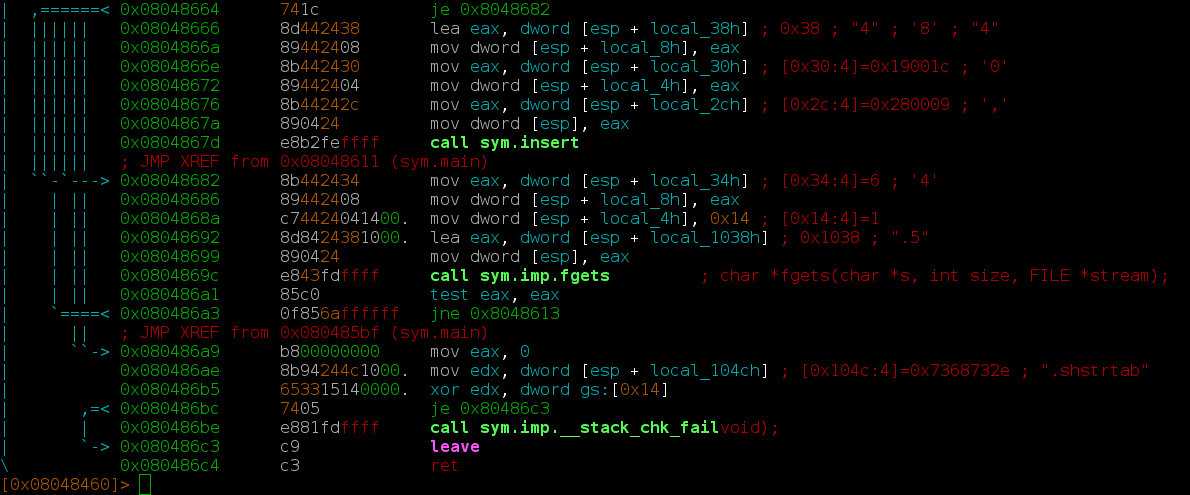
\includegraphics[scale=0.40]{r2.png}
  \caption{Capture d'écran de Radare2}
\end{figure}

\section{Analyse dynamique}

L'analyse dynamique, en opposition à l'analyse statique,
repose donc sur l'exécution du binaire suspect et l'observation
des différentes actions et modifications apportées au système hôte.
Cette technique peut être dangereuse pour l'environnement de travail et
doit être correctement exécutée.

\subsection{Machine virtuelle}

L'élément à étudier peut ne pas correspondre à l'environnement de travail:
un malware Windows ne pourra affecter votre système si celui-ci est un GNU/Linux.
C'est pourquoi il est essentiel de mettre en place
un système de machine virtuelles.\\

De nombreux outils comme \href{http://www.vmware.com/fr.html}{\textit{VMware}}
ou \href{https://www.virtualbox.org/}{\textit{VirtualBox}} (gratuit)
permet de pouvoir virtualiser un grand nombre d'architectures,
sans pour autant modifier son environnement et offre la possibilité de choisir
, de configurer le système qui sera infecté (utile pour forcer certaines
versions du noyau, la persistance de certaines failles de sécurité, \ldots).\\
Un autre avantage à l'utilisation de machines virtuelles
est la capacité de pouvoir utiliser des snapshots. Ces "instantanés" vont
capturer l'état de la machine virtuelle (mémoire, configurations,
état des disques, \ldots) à un moment précis. Les modifications alors apportées
à la machine seront indépendantes du snapshots, préservant l'état de la VM
original. Si l'utilisateur a besoin de revenir en arrière sur ses actions,
il lui suffit de restaurer son snapshot, autant de fois que nécessaire.
Ceci est particulièrement utile lors de l'étude d'un malware, afin de pouvoir
étudier plusieurs fois la phase d'infection ou la première communication avec
un serveur C\&C, par exemple.\\

\subsection{Simulation de réseaux}

Un autre avantage à l'utilisation de machines virtuelles comme
environnement d'étude est la possibilité de relier plusieurs
machines virtuelles entre elles, comme dans un vrai réseau, tout en gardant
le contrôle sur chacune d'elles. Il est alors possible de créer totalement
son environnement, de l'ordonner, de le gérer (création de serveur DNS
par exemple), afin d'adapter l'environnement d'infection au malware et
de pouvoir étudier les communications circulant sur le réseau.\\

\href{http://www.inetsim.org/index.html}{\textit{INetSim}} est un outil
open-source offrant ce service. Celui-ci permet de simuler
des services internet qui sont habituellement utilisés par les malwares dans
un environnement de travail confiné. Parmi les modules proposés et qui peuvent
être utiles, il est possible de trouver la mise en place de service DNS, FTP,
HTTP, Daytime, \ldots

\subsection{Analyse de trafic}

Une fois l'environnement mis en place et que l'élément à analyser pense
communiquer normalement avec l'extérieur, il est bien souvent intéressant
d'observer et d'étudier ces communications. Ceci peut permettre d'inférer ou
de confirmer un comportement vu lors de la lecture de code, ou au contraire,
d'observer une interaction encore inconnue avec du malware avec
son environnement.\\

L'analyse de trafic ethernet peut être effectué à l'aide d'un outil
de capture de paquets libre comme
\href{http://www.tcpdump.org/}{\textit{tcpdump}} ou
\href{https://www.wireshark.org/}{\textit{Wireshark}}, disponibles sur
plusieurs architectures et systèmes. L'utilisateur peut alors utiliser un
filtre (BPF pour tcpdump, par exemple) ou les fonctionnalités de
\textit{Wireshark} afin de disséquer plus simplement les paquets,
de travailler sur des protocoles déjà connus ou encore,
d'en découvrir et de les étudier.\\
Ce type d'étude peut être très pratique lors de la communication avec
un serveur C\&C.

\subsection{Listing des processus}

Une autre facette importante de l'infection à étudier, outre la
communication réseau, est l'état de la machine au cours de l'infection
et une fois celle-ci terminée.\\
La première chose qui vient à l'esprit est donc de regarder les processus
actif et leurs actions. C'est souvent ainsi que l'on remarque une infection,
lorsqu'un processus qui ne devrait pas être présent, l'est.
Ainsi, une connection ssh ouverte depuis l'extérieur, vers la machine alors
que seul un navigateur a été ouvert, peut témoigner de la présence
d'une backdoor.\\

De nombreux outils sont disponibles, nativement, sur les systèmes
d'exploitation, comme \href{https://linux.die.net/man/1/ps}{\textit{ps}} ou
\href{https://linux.die.net/man/1/pstree}{\textit{pstree}} sur Linux.
Mais il existe aussi des outils propriétaires aussi bien utiles, comme
\href{https://process-explorer.fr.softonic.com/}{\textit{Process Explorer}},
sur Windows, proposant des analyses plus
complètes des processus actif sur le système de l'utilisateur.

Quoi de plus naturel que d'ouvrir la liste des processus actifs afin de voir
la consommation en CPU/mémoire, lorsque le système semble plus lent
qu'à son habitude ?

\subsection{Tracing}

Mais il est aussi important de savoir les actions effectuées par le logiciel
suspicieux (et ses différents threads et daemons, s'il y a).\\

En effet, il est possible de tracer les appels systèmes effectués et les signaux
reçus par un exécutable, sous linux, avec la commande
\href{https://technet.microsoft.com/fr-fr/sysinternals/processmonitor.aspx}
     {\textit{strace}}. De même pour Windows, il est possible d'utiliser l'outil
     \href{https://linux.die.net/man/1/strace}{\textit{Process Monitor}},
gratuit, qui se charge d'afficher et de gérer l'état des fichiers du système,
les interactions avec les registres Windows ainsi que l'utilisation et
les appels de DLL.

\subsection{Débugueur}

Enfin, une des étapes de l'analyse de malware consiste à analyser celui-ci
à l'aide d'un débugueur. Ces outils permettent de suivre l'exécution
du malware, pas à pas, si aucune technique anti-debug n'est présente
dans le binaire étudié. Cette technique est particulièrement utile lorsqu'il
s'agit de connaître le contenu d'un prédicat opaque, d'une variable que l'on ne
peut appréhender facilement durant l'analyse statique,
comme lors d'un embranchement dépendant de ce prédicat ou d'une phase de
déchiffrement dépendant d'une variable contenant la clef.\\

Parmi les outils existant, la plupart des outils décrits dans la partie (TODO)
sont des débugueurs. Il peut être aussi utile de citer
\href{https://developer.android.com/studio/command-line/adb.html}{\textit{ADB}}
(Androi Debug Bridge) pour les systèmes android et
\href{http://x64dbg.com/#overview}{\textit{x64dbg}} pour Windows,
qui est open-source.\\
